\section{Events} \label{events}
\subsection{Time elapsed}
 Running tasks at pre-determined rates is desirable in many situations, like sensory data acquisition, low-level servoing, control loops, action planning and system monitoring. As seen in section \ref{addtask}, you can schedule tasks at any interval your design demands, at least, if the time specification is lower than the scheduler tick. When an application consists of several periodic tasks with individual timing constraints, a few points must be taken:

\begin{itemize}
    \item When the time interval of a certain task has elapsed, the scheduler triggers an event (\textit{byTimeElapsed}) that put the task in a \lstinline{qReady} state  (see figure ~\ref{fig:timelag}).
    \item If a task has a finite number iterations, the scheduler will disable the task when the number of iterations reaches the programmed value.
    \item Tasks always have an inherent time-lag that can be noticed even more, when the programmed time-interval is too low (see figure ~\ref{fig:timelag}). In a real-time context, it is important to reduce this time-lag or jitter, to an acceptable level for the application. 
    \medskip
    
    \begin{tcolorbox}
    \HandRight QuarkTS can generally meet a time deadline if you use lightweight code in the callbacks and there is a reduced pool of pending tasks, so it can be considered a soft real-time scheduler, however,  it cannot meet a deadline deterministically like a hard real-time OS.
    \end{tcolorbox}

    \begin{figure}[H]
    \centering
    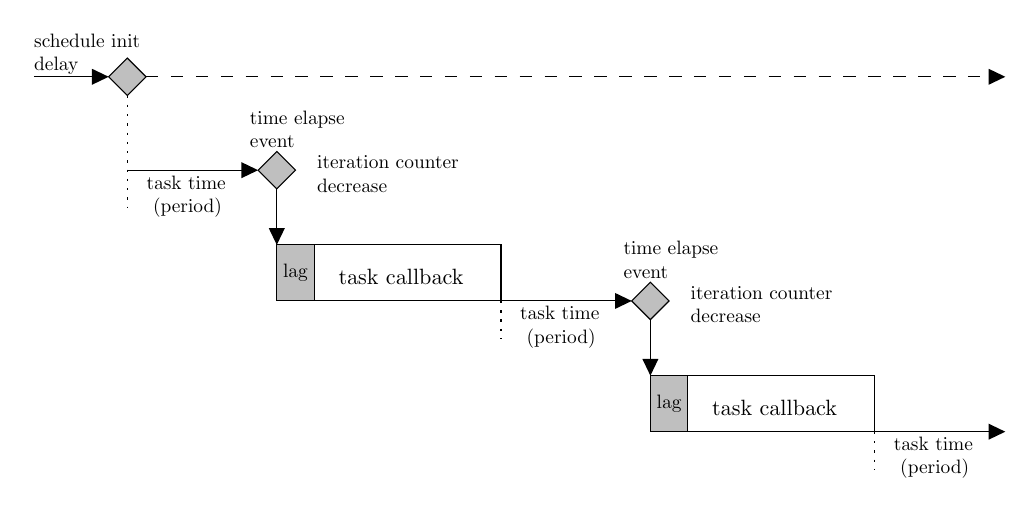
\begin{tikzpicture}[x=0.75pt,y=0.75pt,yscale=-1,xscale=1,scale=0.9]
        \draw  [fill=lightgray,fill opacity=1 ] (130,20) -- (140,30) -- (130,40) -- (120,30) -- cycle ;
        \draw    (80,30) -- (118,30) ;
        \draw [shift={(120,30)}, rotate = 180] [fill=black][line width=0.75]  [draw opacity=0] (8.93,-4.29) -- (0,0) -- (8.93,4.29) -- cycle;
        \draw  [dash pattern={on 4.5pt off 4.5pt}]  (140,30) -- (598,30) ;
        \draw [shift={(600,30)}, rotate = 180] [fill=black][line width=0.75]  [draw opacity=0] (8.93,-4.29) -- (0,0) -- (8.93,4.29) -- cycle;
        \draw  [dash pattern={on 0.84pt off 2.51pt}]  (130,40) -- (130,100) ;
        \draw    (130,80) -- (198,80) ;
        \draw [shift={(200,80)}, rotate = 180] [fill=black][line width=0.75]  [draw opacity=0] (8.93,-4.29) -- (0,0) -- (8.93,4.29) -- cycle;
        \draw  [fill=lightgray,fill opacity=1 ] (210,70) -- (220,80) -- (210,90) -- (200,80) -- cycle ;
        \draw  [fill=lightgray,fill opacity=1 ] (210,120) -- (230,120) -- (230,150) -- (210,150) -- cycle ;
        \draw   (230,120) -- (330,120) -- (330,150) -- (230,150) -- cycle ;
        \draw    (210,90) -- (210,118) ;
        \draw [shift={(210,120)}, rotate = 270] [fill=black][line width=0.75]  [draw opacity=0] (8.93,-4.29) -- (0,0) -- (8.93,4.29) -- cycle;
        \draw  [dash pattern={on 0.84pt off 2.51pt}]  (330,150) -- (330,170) ;
        \draw    (330,150) -- (398,150) ;
        \draw [shift={(400,150)}, rotate = 180] [fill=black][line width=0.75]  [draw opacity=0] (8.93,-4.29) -- (0,0) -- (8.93,4.29) -- cycle;
        \draw  [fill=lightgray,fill opacity=1 ] (410,140) -- (420,150) -- (410,160) -- (400,150) -- cycle ;
        \draw  [fill=lightgray,fill opacity=1 ] (410,190) -- (430,190) -- (430,220) -- (410,220) -- cycle ;
        \draw   (430,190) -- (530,190) -- (530,220) -- (430,220) -- cycle ;
        \draw    (410,160) -- (410,188) ;
        \draw [shift={(410,190)}, rotate = 270] [fill=black][line width=0.75]  [draw opacity=0] (8.93,-4.29) -- (0,0) -- (8.93,4.29) -- cycle;
        \draw  [dash pattern={on 0.84pt off 2.51pt}]  (530,220) -- (530,240) ;
        \draw    (530,220) -- (598,220) ;
        \draw [shift={(600,220)}, rotate = 180] [fill=black][line width=0.75]  [draw opacity=0] (8.93,-4.29) -- (0,0) -- (8.93,4.29) -- cycle;
        \draw (108.5,18) node [scale=0.7] [align=left] {schedule init\\delay};
        \draw (221,58) node [scale=0.7] [align=left] {time elapse\\event};
        \draw (220,135) node [scale=0.7] [align=left] {lag};
        \draw (276.5,137) node [scale=0.8] [align=left] {task callback};
        \draw (269.5,82) node [scale=0.7] [align=left] {iteration counter\\decrease};
        \draw (161.5,94) node [scale=0.7] [align=left] { task time\\ \ (period)};
        \draw (421,128) node [scale=0.7] [align=left] {time elapse\\event};
        \draw (420,205) node [scale=0.7] [align=left] {lag};
        \draw (476.5,207) node [scale=0.8] [align=left] {task callback};
        \draw (469.5,152) node [scale=0.7] [align=left] {iteration counter\\decrease};
        \draw (361.5,164) node [scale=0.7] [align=left] { task time\\ \ (period)};
        \draw (561.5,234) node [scale=0.7] [align=left] { task time\\ \ (period)};
    \end{tikzpicture}
    \caption{Inherit time lag}
    \label{fig:timelag}
\end{figure}

    \item The most significant delay times are produced inside the callbacks. As mentioned before, use short efficient callback methods written for cooperative scheduling.
    \item If two tasks have the same time-interval, the scheduler executes first, the task with the highest priority value (see figure \ref{fig:timelapsed}).

    \begin{figure}[H]
    \centering
        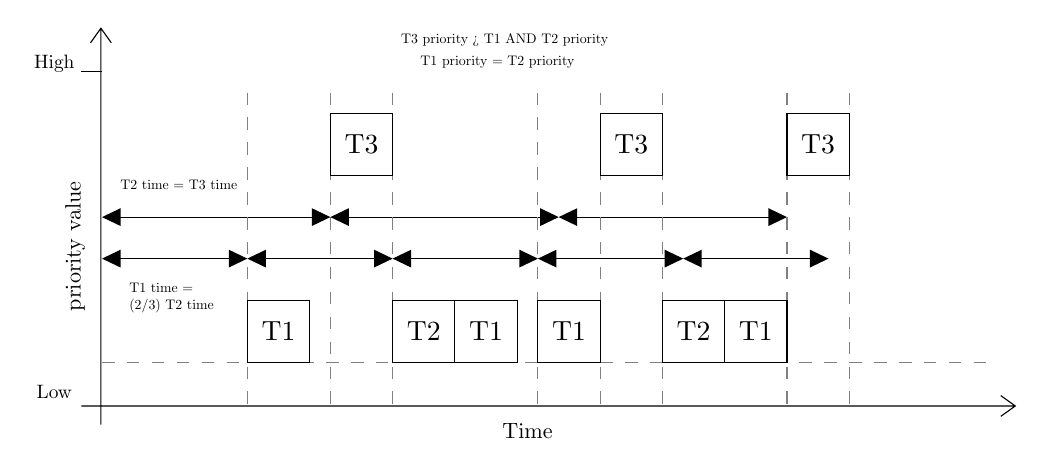
\begin{tikzpicture}[x=0.75pt,y=0.75pt,yscale=-1,xscale=1]
        \draw  (50,241) -- (500,241)(59.45,59) -- (59.45,250) (493,236) -- (500,241) -- (493,246) (54.45,66) -- (59.45,59) -- (64.45,66)  ;
        \draw    (50,80) -- (60,80) ;
        \draw [color=gray  ,draw opacity=1 ] [dash pattern={on 4.5pt off 4.5pt}]  (60,220) -- (490,220) ;
        \draw [color=gray  ,draw opacity=1 ] [dash pattern={on 4.5pt off 4.5pt}]  (170,90) -- (170,240) ;
        \draw    (62,170) -- (128,170) ;
        \draw [shift={(130,170)}, rotate = 180] [fill=black][line width=0.75]  [draw opacity=0] (8.93,-4.29) -- (0,0) -- (8.93,4.29) -- cycle;
        \draw [shift={(60,170)}, rotate = 0] [fill=black][line width=0.75]  [draw opacity=0] (8.93,-4.29) -- (0,0) -- (8.93,4.29) -- cycle ;
        \draw  [fill=white  ,fill opacity=1 ] (230,190) -- (260,190) -- (260,220) -- (230,220) -- cycle ;
        \draw    (62,150) -- (168,150) ;
        \draw [shift={(170,150)}, rotate = 180] [fill=black][line width=0.75][draw opacity=0] (8.93,-4.29) -- (0,0) -- (8.93,4.29) -- cycle;
        \draw [shift={(60,150)}, rotate = 0] [fill=black][line width=0.75]  [draw opacity=0] (8.93,-4.29) -- (0,0) -- (8.93,4.29) -- cycle;
        \draw    (172,150) -- (278,150) ;
        \draw [shift={(280,150)}, rotate = 180] [fill=black][line width=0.75][draw opacity=0] (8.93,-4.29) -- (0,0) -- (8.93,4.29) -- cycle;
        \draw [shift={(170,150)}, rotate = 0] [fill=black][line width=0.75][draw opacity=0] (8.93,-4.29) -- (0,0) -- (8.93,4.29) -- cycle;
        \draw    (282,150) -- (388,150) ;
        \draw [shift={(390,150)}, rotate = 180] [fill=black][line width=0.75]  [draw opacity=0] (8.93,-4.29) -- (0,0) -- (8.93,4.29) -- cycle;
        \draw [shift={(280,150)}, rotate = 0] [fill=black][line width=0.75]  [draw opacity=0] (8.93,-4.29) -- (0,0) -- (8.93,4.29) -- cycle;
        \draw [color=gray  ,draw opacity=1 ] [dash pattern={on 4.5pt off 4.5pt}]  (270,90) -- (270,240) ;
        \draw [color=gray  ,draw opacity=1 ] [dash pattern={on 4.5pt off 4.5pt}]  (390,90) -- (390,240) ;
        \draw [color=gray  ,draw opacity=1 ] [dash pattern={on 4.5pt off 4.5pt}]  (200,90) -- (200,240) ;
        \draw [color=gray  ,draw opacity=1 ] [dash pattern={on 4.5pt off 4.5pt}]  (130,90) -- (130,240) ;
        \draw [color=gray  ,draw opacity=1 ] [dash pattern={on 4.5pt off 4.5pt}]  (300,90) -- (300,240) ;
        \draw    (132,170) -- (198,170) ;
        \draw [shift={(200,170)}, rotate = 180] [fill=black][line width=0.75][draw opacity=0] (8.93,-4.29) -- (0,0) -- (8.93,4.29) -- cycle;
        \draw [shift={(130,170)}, rotate = 0] [fill=black][line width=0.75][draw opacity=0] (8.93,-4.29) -- (0,0) -- (8.93,4.29) -- cycle;
        \draw    (202,170) -- (268,170) ;
        \draw [shift={(270,170)}, rotate = 180] [fill=black][line width=0.75][draw opacity=0] (8.93,-4.29) -- (0,0) -- (8.93,4.29) -- cycle;
        \draw [shift={(200,170)}, rotate = 0] [fill=black][line width=0.75][draw opacity=0] (8.93,-4.29) -- (0,0) -- (8.93,4.29) -- cycle;
        \draw    (272,170) -- (338,170) ;
        \draw [shift={(340,170)}, rotate = 180] [fill=black][line width=0.75][draw opacity=0] (8.93,-4.29) -- (0,0) -- (8.93,4.29) -- cycle;
        \draw [shift={(270,170)}, rotate = 0] [fill=black][line width=0.75][draw opacity=0] (8.93,-4.29) -- (0,0) -- (8.93,4.29) -- cycle;
        \draw    (342,170) -- (408,170) ;
        \draw [shift={(410,170)}, rotate = 180] [fill=black][line width=0.75]  [draw opacity=0] (8.93,-4.29) -- (0,0) -- (8.93,4.29) -- cycle;
        \draw [shift={(340,170)}, rotate = 0] [fill=black  ][line width=0.75]  [draw opacity=0] (8.93,-4.29) -- (0,0) -- (8.93,4.29) -- cycle;
        \draw  [fill=white  ,fill opacity=1 ] (270,190) -- (300,190) -- (300,220) -- (270,220) -- cycle ;
        \draw [color=gray  ,draw opacity=1 ] [dash pattern={on 4.5pt off 4.5pt}]  (330,90) -- (330,240) ;
        \draw  [fill=white  ,fill opacity=1 ] (300,100) -- (330,100) -- (330,130) -- (300,130) -- cycle ;
        \draw  [fill=white  ,fill opacity=1 ] (170,100) -- (200,100) -- (200,130) -- (170,130) -- cycle ;
        \draw  [fill=white  ,fill opacity=1 ] (200,190) -- (230,190) -- (230,220) -- (200,220) -- cycle ;
        \draw [color=gray  ,draw opacity=1 ] [dash pattern={on 4.5pt off 4.5pt}]  (420,90) -- (420,240) ;
        \draw  [fill=white  ,fill opacity=1 ] (330,190) -- (360,190) -- (360,220) -- (330,220) -- cycle ;
        \draw  [fill=white  ,fill opacity=1 ] (390,100) -- (420,100) -- (420,130) -- (390,130) -- cycle ;
        \draw  [fill=white  ,fill opacity=1 ] (130,190) -- (160,190) -- (160,220) -- (130,220) -- cycle ;
        \draw  [fill=white  ,fill opacity=1 ] (360,190) -- (390,190) -- (390,220) -- (360,220) -- cycle ;
        \draw (47,164) node [scale=0.8,rotate=-270] [align=left] {priority value};
        \draw (265,253) node [scale=0.8] [align=left] {Time};
        \draw (37,76) node [scale=0.7] [align=left] {High};
        \draw (37,234) node [scale=0.7] [align=left] {Low};
        \draw (245,205) node  [align=left] {T1};
        \draw (185,115) node  [align=left] {T3};
        \draw (215,205) node  [align=left] {T2};
        \draw (285,205) node  [align=left] {T1};
        \draw (315,115) node  [align=left] {T3};
        \draw (405,115) node  [align=left] {T3};
        \draw (145,205) node  [align=left] {T1};
        \draw (97,134.5) node [scale=0.5] [align=left] {T2 time = T3 time};
        \draw (254,64.5) node [scale=0.5] [align=left] {T3 priority > T1 AND T2 priority};
        \draw (250.5,75.5) node [scale=0.5] [align=left] {T1 priority = T2 priority};
        \draw (93.5,189) node [scale=0.5] [align=left] {T1 time = \\(2/3) T2 time};
        \draw (345,205) node  [align=left] {T2};
        \draw (375,205) node  [align=left] {T1};
    \end{tikzpicture}
    \caption{Priority scheduling example with three (3) tasks attached triggered by time-elapsed events}
    \label{fig:timelapsed}
\end{figure}

\end{itemize}
\subsection{Asynchronous events and inter-task communication}
Applications existing in heavy environments require tasks and ISR interacting with each other, forcing the application to implement some event model.
Here, we understand events, as any identifiable occurrence that has significance for the embedded system. As such, events include changes in hardware, user-generated actions or messages coming from components of the application itself.

\begin{figure}[H]
    \centering
    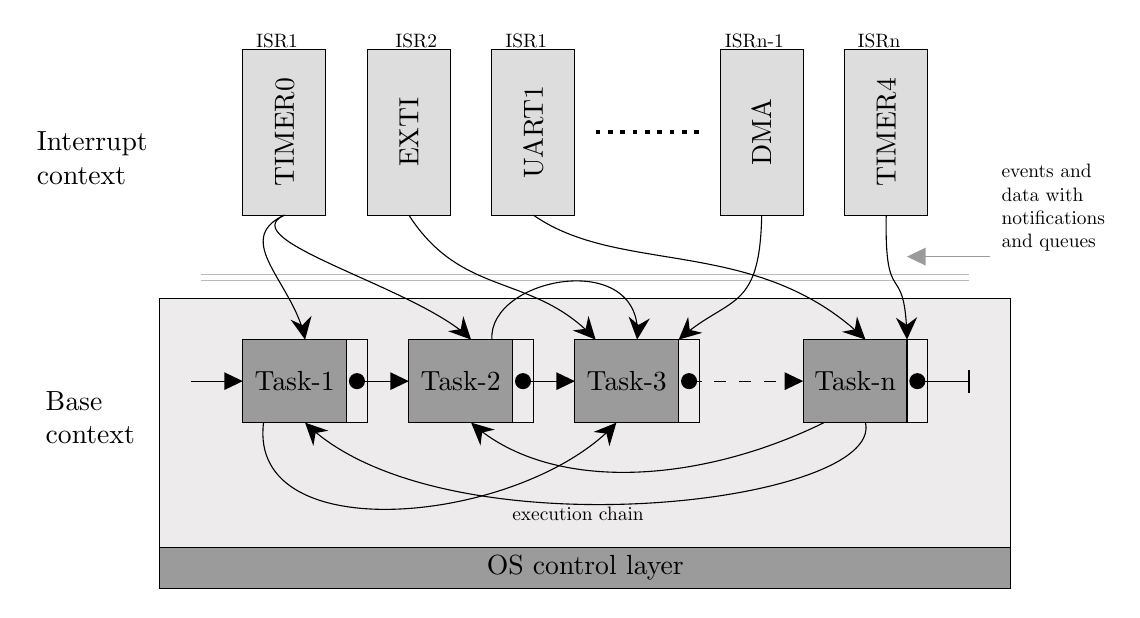
\begin{tikzpicture}[x=0.75pt,y=0.75pt,yscale=-1,xscale=1,scale=1]
        \draw  [fill={rgb, 255:red, 237; green, 235; blue, 235 }  ,fill opacity=1 ] (170,200) -- (580,200) -- (580,340) -- (170,340) -- cycle ;
        \draw  [fill={rgb, 255:red, 222; green, 221; blue, 221 }  ,fill opacity=1 ] (210,80) -- (250,80) -- (250,160) -- (210,160) -- cycle ;
        \draw  [fill={rgb, 255:red, 222; green, 221; blue, 221 }  ,fill opacity=1 ] (270,80) -- (310,80) -- (310,160) -- (270,160) -- cycle ;
        \draw  [fill={rgb, 255:red, 222; green, 221; blue, 221 }  ,fill opacity=1 ] (330,80) -- (370,80) -- (370,160) -- (330,160) -- cycle ;
        \draw  [fill={rgb, 255:red, 222; green, 221; blue, 221 }  ,fill opacity=1 ] (440,80) -- (480,80) -- (480,160) -- (440,160) -- cycle ;
        \draw  [fill={rgb, 255:red, 222; green, 221; blue, 221 }  ,fill opacity=1 ] (500,80) -- (540,80) -- (540,160) -- (500,160) -- cycle ;
        \draw [line width=1.5]  [dash pattern={on 1.69pt off 2.76pt}]  (380,120) -- (430,120) ;
        \draw  [fill={rgb, 255:red, 155; green, 155; blue, 155 }  ,fill opacity=1 ] (210,220) -- (260,220) -- (260,260) -- (210,260) -- cycle ;
        \draw   (260,220) -- (270,220) -- (270,260) -- (260,260) -- cycle ;
        \draw  [fill={rgb, 255:red, 155; green, 155; blue, 155 }  ,fill opacity=1 ] (290,220) -- (340,220) -- (340,260) -- (290,260) -- cycle ;
        \draw   (340,220) -- (350,220) -- (350,260) -- (340,260) -- cycle ;
        \draw  [fill={rgb, 255:red, 155; green, 155; blue, 155 }  ,fill opacity=1 ] (370,220) -- (420,220) -- (420,260) -- (370,260) -- cycle ;
        \draw   (420,220) -- (430,220) -- (430,260) -- (420,260) -- cycle ;
        \draw  [fill={rgb, 255:red, 155; green, 155; blue, 155 }  ,fill opacity=1 ] (480,220) -- (530,220) -- (530,260) -- (480,260) -- cycle ;
        \draw   (530,220) -- (540,220) -- (540,260) -- (530,260) -- cycle ;
        \draw    (265,240) -- (288,240) ;
        \draw [shift={(290,240)}, rotate = 180] [fill={rgb, 255:red, 0; green, 0; blue, 0 }  ][line width=0.75]  [draw opacity=0] (8.93,-4.29) -- (0,0) -- (8.93,4.29) -- cycle    ;
        \draw [shift={(265,240)}, rotate = 0] [color={rgb, 255:red, 0; green, 0; blue, 0 }  ][fill={rgb, 255:red, 0; green, 0; blue, 0 }  ][line width=0.75]      (0, 0) circle [x radius= 3.35, y radius= 3.35]   ;
        \draw    (345,240) -- (368,240) ;
        \draw [shift={(370,240)}, rotate = 180] [fill={rgb, 255:red, 0; green, 0; blue, 0 }  ][line width=0.75]  [draw opacity=0] (8.93,-4.29) -- (0,0) -- (8.93,4.29) -- cycle    ;
        \draw [shift={(345,240)}, rotate = 0] [color={rgb, 255:red, 0; green, 0; blue, 0 }  ][fill={rgb, 255:red, 0; green, 0; blue, 0 }  ][line width=0.75]      (0, 0) circle [x radius= 3.35, y radius= 3.35]   ;
        \draw    (535,240) -- (560,240) ;
        \draw [shift={(560,240)}, rotate = 180] [color={rgb, 255:red, 0; green, 0; blue, 0 }  ][line width=0.75]    (0,5.59) -- (0,-5.59)   ;
        \draw [shift={(535,240)}, rotate = 0] [color={rgb, 255:red, 0; green, 0; blue, 0 }  ][fill={rgb, 255:red, 0; green, 0; blue, 0 }  ][line width=0.75]      (0, 0) circle [x radius= 3.35, y radius= 3.35]   ;
        \draw  [dash pattern={on 4.5pt off 4.5pt}]  (425,240) -- (478,240) ;
        \draw [shift={(480,240)}, rotate = 180] [fill={rgb, 255:red, 0; green, 0; blue, 0 }  ][line width=0.75]  [draw opacity=0] (8.93,-4.29) -- (0,0) -- (8.93,4.29) -- cycle    ;
        \draw [shift={(425,240)}, rotate = 0] [color={rgb, 255:red, 0; green, 0; blue, 0 }  ][fill={rgb, 255:red, 0; green, 0; blue, 0 }  ][line width=0.75]      (0, 0) circle [x radius= 3.35, y radius= 3.35]   ;
        \draw    (185,240) -- (208,240) ;
        \draw [shift={(210,240)}, rotate = 180] [fill={rgb, 255:red, 0; green, 0; blue, 0 }  ][line width=0.75]  [draw opacity=0] (8.93,-4.29) -- (0,0) -- (8.93,4.29) -- cycle    ;
        \draw [color={rgb, 255:red, 189; green, 185; blue, 185 }  ,draw opacity=1 ]   (190,188.5) -- (560,188.5)(190,191.5) -- (560,191.5) ;
        \draw    (230,160) .. controls (204.63,171.97) and (233.89,192.37) .. (239.68,218.4) ;
        \draw [shift={(240,220)}, rotate = 259.65] [fill={rgb, 255:red, 0; green, 0; blue, 0 }  ][line width=0.75]  [draw opacity=0] (10.72,-5.15) -- (0,0) -- (10.72,5.15) -- (7.12,0) -- cycle    ;
        \draw    (230,160) .. controls (204.5,172.03) and (293.37,194.79) .. (318.88,218.9) ;
        \draw [shift={(320,220)}, rotate = 225.74] [fill={rgb, 255:red, 0; green, 0; blue, 0 }  ][line width=0.75]  [draw opacity=0] (10.72,-5.15) -- (0,0) -- (10.72,5.15) -- (7.12,0) -- cycle    ;
        \draw    (330,220) .. controls (328.14,190.03) and (401.85,176) .. (400.13,218.04) ;
        \draw [shift={(400,220)}, rotate = 275.28] [fill={rgb, 255:red, 0; green, 0; blue, 0 }  ][line width=0.75]  [draw opacity=0] (10.72,-5.15) -- (0,0) -- (10.72,5.15) -- (7.12,0) -- cycle    ;
        \draw    (510,260) .. controls (519.06,299.2) and (307.24,324.14) .. (240.99,260.96) ;
        \draw [shift={(240,260)}, rotate = 404.68] [fill={rgb, 255:red, 0; green, 0; blue, 0 }  ][line width=0.75]  [draw opacity=0] (10.72,-5.15) -- (0,0) -- (10.72,5.15) -- (7.12,0) -- cycle    ;
        \draw    (350,160) .. controls (391.9,189.34) and (457.45,169.68) .. (509.22,219.25) ;
        \draw [shift={(510,220)}, rotate = 224.23] [fill={rgb, 255:red, 0; green, 0; blue, 0 }  ][line width=0.75]  [draw opacity=0] (10.72,-5.15) -- (0,0) -- (10.72,5.15) -- (7.12,0) -- cycle    ;
        \draw    (460,160) .. controls (459.13,206.53) and (444.7,198.82) .. (421.44,218.74) ;
        \draw [shift={(420,220)}, rotate = 318.25] [fill={rgb, 255:red, 0; green, 0; blue, 0 }  ][line width=0.75]  [draw opacity=0] (10.72,-5.15) -- (0,0) -- (10.72,5.15) -- (7.12,0) -- cycle    ;
        \draw    (220,260) .. controls (212.19,321.86) and (343.44,308.76) .. (388.66,261.44) ;
        \draw [shift={(390,260)}, rotate = 492.15] [fill={rgb, 255:red, 0; green, 0; blue, 0 }  ][line width=0.75]  [draw opacity=0] (10.72,-5.15) -- (0,0) -- (10.72,5.15) -- (7.12,0) -- cycle    ;
        \draw    (290,160) .. controls (315.72,199.88) and (349.09,187.86) .. (378.65,218.57) ;
        \draw [shift={(380,220)}, rotate = 227.41] [fill={rgb, 255:red, 0; green, 0; blue, 0 }  ][line width=0.75]  [draw opacity=0] (10.72,-5.15) -- (0,0) -- (10.72,5.15) -- (7.12,0) -- cycle    ;
        \draw  [fill={rgb, 255:red, 155; green, 155; blue, 155 }  ,fill opacity=1 ] (170,320) -- (580,320) -- (580,340) -- (170,340) -- cycle ;
        \draw    (520,160) .. controls (519.12,206.77) and (528.81,180.22) .. (529.95,218.22) ;
        \draw [shift={(530,220)}, rotate = 268.74] [fill={rgb, 255:red, 0; green, 0; blue, 0 }  ][line width=0.75]  [draw opacity=0] (10.72,-5.15) -- (0,0) -- (10.72,5.15) -- (7.12,0) -- cycle    ;
        \draw [color={rgb, 255:red, 155; green, 155; blue, 155 }  ,draw opacity=1 ]   (570,180) -- (532,180) ;
        \draw [shift={(530,180)}, rotate = 360] [fill={rgb, 255:red, 155; green, 155; blue, 155 }  ,fill opacity=1 ][line width=0.75]  [draw opacity=0] (8.93,-4.29) -- (0,0) -- (8.93,4.29) -- cycle    ;
        \draw    (490,260) .. controls (430.71,289.1) and (359.55,294.29) .. (321.15,261.02) ;
        \draw [shift={(320,260)}, rotate = 402.07] [fill={rgb, 255:red, 0; green, 0; blue, 0 }  ][line width=0.75]  [draw opacity=0] (10.72,-5.15) -- (0,0) -- (10.72,5.15) -- (7.12,0) -- cycle    ;
        \draw (230,120) node [rotate=-270] [align=left] {TIMER0};
        \draw (290,120) node [rotate=-270] [align=left] {EXTI};
        \draw (350,120) node [rotate=-270] [align=left] {UART1};
        \draw (460,120) node [rotate=-270] [align=left] {DMA};
        \draw (520,120) node [rotate=-270] [align=left] {TIMER4};
        \draw (235,240) node  [align=left] {Task-1};
        \draw (315,240) node  [align=left] {Task-2};
        \draw (395,240) node  [align=left] {Task-3};
        \draw (505,240) node  [align=left] {Task-n};
        \draw (226.5,76) node [scale=0.7] [align=left] {ISR1};
        \draw (293.5,76) node [scale=0.7] [align=left] {ISR2};
        \draw (346.5,76) node [scale=0.7] [align=left] {ISR1};
        \draw (516.5,76) node [scale=0.7] [align=left] {ISRn};
        \draw (456.5,76) node [scale=0.7] [align=left] {ISRn-1};
        \draw (136.5,257.5) node  [align=left] {Base \\context};
        \draw (137.5,132.5) node  [align=left] {Interrupt \\context};
        \draw (375,330) node  [align=left] {OS control layer};
        \draw (371.5,304) node [scale=0.7] [align=left] {execution chain};
        \draw (600.5,156.5) node [scale=0.7] [align=left] {events and\\data with\\notifications\\and queues};
    \end{tikzpicture}
    \caption{Heavy cooperative environment}
    \label{fig:heavyenvy}
\end{figure}

As shown in figure 5, two main scenarios are presented, \textit{ISR-to-task} and \textit{task-to-task} interaction.  When using interrupts to catch external events, it is expected to be handled with fast and lightweight code to reduce the variable ISR overhead introduced by the code itself. If too much overhead is used inside an ISR, the system will tend to lose future events. In some specific situations, the best approach is to synchronize the ISR with a task to leave the heavy job in the base-level instead of the interrupt-level, this is also called  \textit{Deferred Interrupt Handling}.

The other scenario is when a task is performing a specific job and another task must be awakened to perform some activities when the other task finishes.
\medskip

Both scenarios require some ways in which tasks can communicate with each other.
For this, the OS does not impose any specific event processing strategy to the application designer but does provide features that allow the chosen strategy to be implemented in a simple and maintainable way. From the OS perspective, these features are just sources of asynchronous events with specific triggers and related data. 
\medskip

The OS provides the following features for task communication:

\subsubsection{Notifications} \label{osnotifications}
The notifications allow tasks to interact with other tasks and to synchronize with ISRs without the need of intermediate variables or separate communication objects. By using notifications, a task or ISR can launch another task sending an event and related data to the receiving task.  This is depicted in figure \ref{fig:simplenotifications}.

\begin{figure}[H]
    \centering
    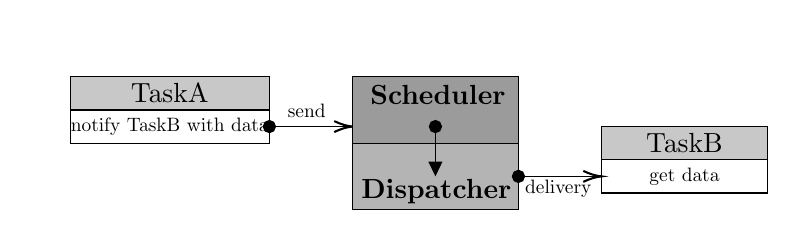
\begin{tikzpicture}[x=0.75pt,y=0.75pt,scale=0.8, yscale=-1]
\draw   (140,110) -- (260,110) -- (260,130) -- (140,130) -- cycle ;
\draw    (260,120) -- (308,120) ;
\draw [shift={(310,120)}, rotate = 180] [color={rgb, 255:red, 0; green, 0; blue, 0 }  ][line width=0.75]    (10.93,-3.29) .. controls (6.95,-1.4) and (3.31,-0.3) .. (0,0) .. controls (3.31,0.3) and (6.95,1.4) .. (10.93,3.29)   ;
\draw [shift={(260,120)}, rotate = 0] [color={rgb, 255:red, 0; green, 0; blue, 0 }  ][fill={rgb, 255:red, 0; green, 0; blue, 0 }  ][line width=0.75]      (0, 0) circle [x radius= 3.35, y radius= 3.35]   ;
\draw  [fill={rgb, 255:red, 200; green, 200; blue, 200 }  ,fill opacity=1 ] (140,90) -- (260,90) -- (260,110) -- (140,110) -- cycle ;
\draw  [fill={rgb, 255:red, 155; green, 155; blue, 155 }  ,fill opacity=1 ] (310,90) -- (410,90) -- (410,130) -- (310,130) -- cycle ;
\draw  [fill={rgb, 255:red, 180; green, 180; blue, 180 }  ,fill opacity=1 ] (310,130) -- (410,130) -- (410,170) -- (310,170) -- cycle ;
\draw    (360,120) -- (360,148) ;
\draw [shift={(360,150)}, rotate = 270] [fill={rgb, 255:red, 0; green, 0; blue, 0 }  ][line width=0.75]  [draw opacity=0] (8.93,-4.29) -- (0,0) -- (8.93,4.29) -- cycle    ;
\draw [shift={(360,120)}, rotate = 90] [color={rgb, 255:red, 0; green, 0; blue, 0 }  ][fill={rgb, 255:red, 0; green, 0; blue, 0 }  ][line width=0.75]      (0, 0) circle [x radius= 3.35, y radius= 3.35]   ;
\draw    (410,150) -- (458,150) ;
\draw [shift={(460,150)}, rotate = 180] [color={rgb, 255:red, 0; green, 0; blue, 0 }  ][line width=0.75]    (10.93,-3.29) .. controls (6.95,-1.4) and (3.31,-0.3) .. (0,0) .. controls (3.31,0.3) and (6.95,1.4) .. (10.93,3.29)   ;
\draw [shift={(410,150)}, rotate = 0] [color={rgb, 255:red, 0; green, 0; blue, 0 }  ][fill={rgb, 255:red, 0; green, 0; blue, 0 }  ][line width=0.75]      (0, 0) circle [x radius= 3.35, y radius= 3.35]   ;
\draw   (460,140) -- (560,140) -- (560,160) -- (460,160) -- cycle ;
\draw  [fill={rgb, 255:red, 200; green, 200; blue, 200 }  ,fill opacity=1 ] (460,120) -- (560,120) -- (560,140) -- (460,140) -- cycle ;
\draw (200,100) node  [align=left] {TaskA};
\draw (120,66) node  [align=left] {};
\draw (361.5,101) node  [align=left] {\textbf{Scheduler}};
% Text Node
\draw (200,120) node [scale=0.7] [align=left] {notify TaskB with data};
% Text Node
\draw (282.5,110.5) node [scale=0.7] [align=left] {send};
% Text Node
\draw (360.5,159) node  [align=left] {\textbf{Dispatcher}};
% Text Node
\draw (434,157.5) node [scale=0.7] [align=left] {delivery};
% Text Node
\draw (510,130) node  [align=left] {TaskB};
% Text Node
\draw (500,146) node  [align=left] {};
% Text Node
\draw (510,150) node [scale=0.7] [align=left] {get data};


\end{tikzpicture}


    \caption{A notification used to send an event directly from one task to another}
    \label{fig:simplenotifications}
\end{figure}




\paragraph{Simple notifications:}
Each task node has a 32-bit notification value which is initialized to zero when a task is added to the scheme. The API \lstinline{qTask_Notification_Send()} \index{\lstinline{qTask_Notification_Send}} is used to send an event directly updating the receiving task's notification value increasing it by one. As long as the scheduler sees a non-zero value, the task will be changed to a \textit{qReady} state and eventually, the dispatcher will launch the task according to the execution chain. After served, the notification value is later decreased.

\begin{lstlisting}[style=CStyle]
qBool_t qTask_Notification_Send( qTask_t * const Task, void* eventdata )
\end{lstlisting}

\subsubsection*{Parameters}
\begin{itemize}
    \item \lstinline{Task} : The pointer of the task node to which the notification is being sent 
    \item \lstinline{EventData} : Specific event user-data. 
\end{itemize}

\subsubsection*{Return value:}

\lstinline{qTrue} if the notification  has been sent, or \lstinline{qFalse} if the notification value reaches its max value. 

\begin{tcolorbox}
\HandRight Sending simple notifications using \lstinline{qTask_Notification_Send()} is interrupt-safe, however, this only catches one event per task because the API overwrites the associated data.
\end{tcolorbox}

\paragraph{Queued notifications}
 : If the application notifies multiple events to the same task, queued notifications are the right solution instead of using simple notifications.

Here, the \lstinline{qTask_Notification_Queue()} \index{\lstinline{qTask_Notification_Queue}} take advantage of the scheduler FIFO priority-queue. 
This kind of queue, is somewhat similar to a standard queue, with an important distinction: when a notification is sent, the task is added to the queue with the corresponding priority level, and will be later removed from the queue with the highest priority task first  \cite{cormen}. That is, the tasks are (conceptually) stored in the queue in priority order instead of the insertion order. If two tasks with the same priority are notified, they are served in the FIFO form according to their order inside the queue. Figure \ref{fig:prioqueue} illustrates this behavior.

\begin{figure}[H]
    \centering
    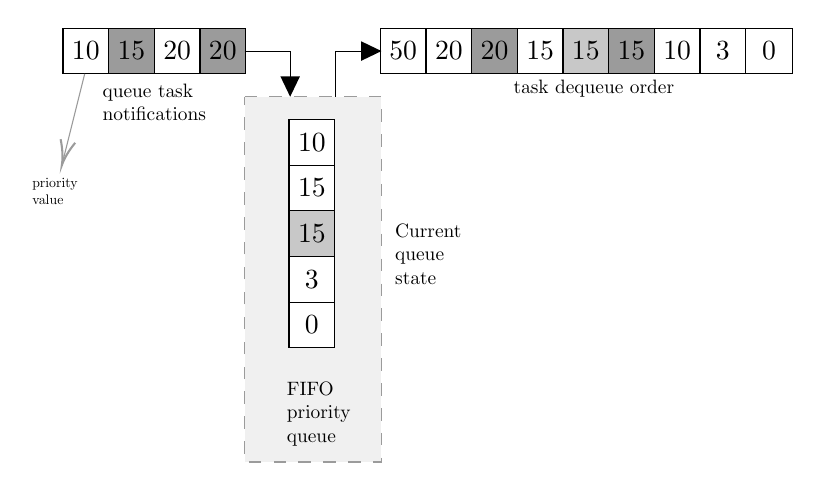
\begin{tikzpicture}[x=0.75pt,y=0.75pt,yscale=-1,xscale=1, scale=1.1]
        \draw   (100.5,50) -- (120.5,50) -- (120.5,70) -- (100.5,70) -- cycle ;
        \draw  [fill={rgb, 255:red, 155; green, 155; blue, 155 }  ,fill opacity=1 ] (120.5,50) -- (140.5,50) -- (140.5,70) -- (120.5,70) -- cycle ;
        \draw   (140.5,50) -- (160.5,50) -- (160.5,70) -- (140.5,70) -- cycle ;
        \draw  [fill={rgb, 255:red, 155; green, 155; blue, 155 }  ,fill opacity=1 ] (160.5,50) -- (180.5,50) -- (180.5,70) -- (160.5,70) -- cycle ;
        \draw   (239.5,50) -- (259.5,50) -- (259.5,70) -- (239.5,70) -- cycle ;
        \draw  [fill={rgb, 255:red, 255; green, 255; blue, 255 }  ,fill opacity=1 ] (259.5,50) -- (279.5,50) -- (279.5,70) -- (259.5,70) -- cycle ;
        \draw   (299.5,50) -- (319.5,50) -- (319.5,70) -- (299.5,70) -- cycle ;
        \draw  [fill={rgb, 255:red, 155; green, 155; blue, 155 }  ,fill opacity=1 ] (279.5,50) -- (299.5,50) -- (299.5,70) -- (279.5,70) -- cycle ;
        \draw  [color={rgb, 255:red, 155; green, 155; blue, 155 }  ,draw opacity=1 ][fill={rgb, 255:red, 240; green, 240; blue, 240 }  ,fill opacity=1 ][dash pattern={on 4.5pt off 4.5pt}] (180,80) -- (240,80) -- (240,240) -- (180,240) -- cycle ;
        \draw    (180,60) -- (200,60) -- (200,78) ;
        \draw [shift={(200,80)}, rotate = 270] [fill={rgb, 255:red, 0; green, 0; blue, 0 }  ][line width=0.75]  [draw opacity=0] (8.93,-4.29) -- (0,0) -- (8.93,4.29) -- cycle;
        \draw  [fill={rgb, 255:red, 200; green, 200; blue, 200 }  ,fill opacity=1 ] (319.5,50) -- (339.5,50) -- (339.5,70) -- (319.5,70) -- cycle ;
        \draw  [fill={rgb, 255:red, 155; green, 155; blue, 155 }  ,fill opacity=1 ] (339.5,50) -- (359.5,50) -- (359.5,70) -- (339.5,70) -- cycle ;
        \draw   (359.5,50) -- (379.5,50) -- (379.5,70) -- (359.5,70) -- cycle ;
        \draw  [fill={rgb, 255:red, 255; green, 255; blue, 255 }  ,fill opacity=1 ] (379.5,50) -- (399.5,50) -- (399.5,70) -- (379.5,70) -- cycle ;
        \draw  [fill={rgb, 255:red, 255; green, 255; blue, 255 }  ,fill opacity=1 ] (399.5,50) -- (420,50) -- (420,70) -- (399.5,70) -- cycle ;
        \draw    (220,80) -- (220,60) -- (238,60) ;
        \draw [shift={(240,60)}, rotate = 180] [fill={rgb, 255:red, 0; green, 0; blue, 0 }  ][line width=0.75]  [draw opacity=0] (8.93,-4.29) -- (0,0) -- (8.93,4.29) -- cycle;
        \draw [color={rgb, 255:red, 155; green, 155; blue, 155 }  ,draw opacity=1 ]   (110,70) -- (100.49,108.06) ;
        \draw [shift={(100,110)}, rotate = 284.04] [color={rgb, 255:red, 155; green, 155; blue, 155 }  ,draw opacity=1 ][line width=0.75]    (10.93,-3.29) .. controls (6.95,-1.4) and (3.31,-0.3) .. (0,0) .. controls (3.31,0.3) and (6.95,1.4) .. (10.93,3.29)   ;
        \draw  [fill={rgb, 255:red, 255; green, 255; blue, 255 }  ,fill opacity=1 ] (199.5,90) -- (219.5,90) -- (219.5,110) -- (199.5,110) -- cycle ;
        \draw  [fill={rgb, 255:red, 255; green, 255; blue, 255 }  ,fill opacity=1 ] (199.5,110) -- (219.5,110) -- (219.5,130) -- (199.5,130) -- cycle ;
        \draw  [fill={rgb, 255:red, 200; green, 200; blue, 200 }  ,fill opacity=1 ] (199.5,130) -- (219.5,130) -- (219.5,150) -- (199.5,150) -- cycle ;
        \draw  [fill={rgb, 255:red, 255; green, 255; blue, 255 }  ,fill opacity=1 ] (199.5,150) -- (219.5,150) -- (219.5,170) -- (199.5,170) -- cycle ;
        \draw  [fill={rgb, 255:red, 255; green, 255; blue, 255 }  ,fill opacity=1 ] (199.5,170) -- (219.5,170) -- (219.5,190) -- (199.5,190) -- cycle ;
        \draw (110.5,60) node  [align=left] {10};
        \draw (130.5,60) node  [align=left] {15};
        \draw (150.5,60) node  [align=left] {20};
        \draw (170.5,60) node  [align=left] {20};
        \draw (249.5,60) node  [align=left] {50};
        \draw (269.5,60) node  [align=left] {20};
        \draw (289.5,60) node  [align=left] {20};
        \draw (309.5,60) node  [align=left] {15};
        \draw (369.5,60) node  [align=left] {10};
        \draw (329.5,60) node  [align=left] {15};
        \draw (349.5,60) node  [align=left] {15};
        \draw (389.5,60) node  [align=left] {3};
        \draw (409.75,60) node  [align=left] {0};
        \draw (260.5,149) node [scale=0.7] [align=left] {Current\\queue\\state};
        \draw (333,76.5) node [scale=0.7] [align=left] {task dequeue order};
        \draw (140.5,82.5) node [scale=0.7] [align=left] {queue task \\notifications};
        \draw (97,121.5) node [scale=0.5] [align=left] {priority\\value};
        \draw (209.5,100) node  [align=left] {10};
        \draw (209.5,120) node  [align=left] {15};
        \draw (209.5,140) node  [align=left] {15};
        \draw (209.5,160) node  [align=left] {3};
        \draw (209.5,180) node  [align=left] {0};
        \draw (212.5,219) node [scale=0.7] [align=left] {FIFO\\priority\\queue};
    \end{tikzpicture}
    \caption{Priority-queue behavior}
    \label{fig:prioqueue}
\end{figure}

The scheduler always checks the queue state first, being this event the one with more precedence among the others. If the queue has elements, the scheduler algorithm will extract the data and the corresponding task will be launched with the trigger flag set in \textit{byNotificationQueued}. 
\medskip

\begin{lstlisting}[style=CStyle]
qBool_t qTask_Notification_Queue( qTask_t * const Task, void* eventdata )
\end{lstlisting}

\subsubsection*{Parameters}
\begin{itemize}
    \item \lstinline{Task} : The pointer of the task node to which the notification is being sent 
    \item \lstinline{EventData} : Specific event user-data. 
\end{itemize}

\subsubsection*{Return value:}

\lstinline{qTrue} if the notification  has been inserted in the queue, or \lstinline{qFalse} if an error occurred or the queue exceeds the size. 
\medskip
\begin{tcolorbox}
\HandRight Among all the provided events, queued notifications have the highest precedence.
\end{tcolorbox}


Figure ~\ref{fig:queueexample}, shows a cooperative environment with five tasks. Initially, the scheduler activates \lstinline{Task-E}, then, this task enqueues data to \lstinline{Task-A} and \lstinline{Task-B} respectively using the \lstinline{qTask_Notification_Queue()} function. In the next scheduler cycle, the scheduler realizes that the priority-queue is not empty, generating an activation over the task located at the beginning of the queue. In this case, \lstinline{Task-A} will be launched and its respective data will be extracted from the queue. However, \lstinline{Task-A} also enqueues data to \lstinline{Task-C} and \lstinline{Task-D}. As mentioned previously, this is a priority-queue, so the scheduler makes a new reordering. In this context, the next queue extraction will be for \lstinline{Task-D}, \lstinline{Task-C}, and \lstinline{Task-B} sequentially.

\begin{figure}[H]
    \centering
    \begin{tikzpicture}[x=0.75pt,y=0.75pt,yscale=-1,xscale=1,scale=0.94]
        \draw  [fill={rgb, 255:red, 155; green, 155; blue, 155 }  ,fill opacity=1 ] (360,110) -- (380,110) -- (380,130) -- (360,130) -- cycle ;
        \draw  [fill={rgb, 255:red, 155; green, 155; blue, 155 }  ,fill opacity=1 ] (380,110) -- (400,110) -- (400,130) -- (380,130) -- cycle ;
        \draw   (400,110) -- (420,110) -- (420,130) -- (400,130) -- cycle ;
        \draw   (420,110) -- (440,110) -- (440,130) -- (420,130) -- cycle ;
        \draw   (440,110) -- (460,110) -- (460,130) -- (440,130) -- cycle ;
        \draw   (100,120) -- (310,120) -- (310,170) -- (100,170) -- cycle ;
        \draw  [fill={rgb, 255:red, 155; green, 155; blue, 155 }  ,fill opacity=1 ] (120,136) .. controls (120,138.21) and (118.21,140) .. (116,140) -- (100,140) -- (100,120) -- (120,120) -- cycle ;
        \draw  [fill={rgb, 255:red, 155; green, 155; blue, 155 }  ,fill opacity=1 ] (360,180) -- (380,180) -- (380,200) -- (360,200) -- cycle ;
        \draw  [fill={rgb, 255:red, 155; green, 155; blue, 155 }  ,fill opacity=1 ] (380,180) -- (400,180) -- (400,200) -- (380,200) -- cycle ;
        \draw  [fill={rgb, 255:red, 155; green, 155; blue, 155 }  ,fill opacity=1 ] (400,180) -- (420,180) -- (420,200) -- (400,200) -- cycle ;
        \draw   (420,180) -- (440,180) -- (440,200) -- (420,200) -- cycle ;
        \draw   (440,180) -- (460,180) -- (460,200) -- (440,200) -- cycle ;
        \draw  [fill={rgb, 255:red, 200; green, 200; blue, 200 }  ,fill opacity=1 ] (100,190) -- (310,190) -- (310,240) -- (100,240) -- cycle ;
        \draw  [fill={rgb, 255:red, 155; green, 155; blue, 155 }  ,fill opacity=1 ] (120,206) .. controls (120,208.21) and (118.21,210) .. (116,210) -- (100,210) -- (100,190) -- (120,190) -- cycle ;
        \draw  [fill={rgb, 255:red, 200; green, 200; blue, 200 }  ,fill opacity=1 ] (100,260) -- (310,260) -- (310,290) -- (100,290) -- cycle ;
        \draw  [fill={rgb, 255:red, 155; green, 155; blue, 155 }  ,fill opacity=1 ] (120,276) .. controls (120,278.21) and (118.21,280) .. (116,280) -- (100,280) -- (100,260) -- (120,260) -- cycle ;
        \draw  [fill={rgb, 255:red, 200; green, 200; blue, 200 }  ,fill opacity=1 ] (100,310) -- (310,310) -- (310,340) -- (100,340) -- cycle ;
        \draw  [fill={rgb, 255:red, 155; green, 155; blue, 155 }  ,fill opacity=1 ] (120,326) .. controls (120,328.21) and (118.21,330) .. (116,330) -- (100,330) -- (100,310) -- (120,310) -- cycle ;
        \draw  [fill={rgb, 255:red, 200; green, 200; blue, 200 }  ,fill opacity=1 ] (100,360) -- (310,360) -- (310,390) -- (100,390) -- cycle ;
        \draw  [fill={rgb, 255:red, 155; green, 155; blue, 155 }  ,fill opacity=1 ] (120,376) .. controls (120,378.21) and (118.21,380) .. (116,380) -- (100,380) -- (100,360) -- (120,360) -- cycle ;
        \draw  [fill={rgb, 255:red, 155; green, 155; blue, 155 }  ,fill opacity=1 ] (360,250) -- (380,250) -- (380,270) -- (360,270) -- cycle ;
        \draw  [fill={rgb, 255:red, 155; green, 155; blue, 155 }  ,fill opacity=1 ] (380,250) -- (400,250) -- (400,270) -- (380,270) -- cycle ;
        \draw   (400,250) -- (420,250) -- (420,270) -- (400,270) -- cycle ;
        \draw   (420,250) -- (440,250) -- (440,270) -- (420,270) -- cycle ;
        \draw   (440,250) -- (460,250) -- (460,270) -- (440,270) -- cycle ;
        \draw  [fill={rgb, 255:red, 155; green, 155; blue, 155 }  ,fill opacity=1 ] (360,300) -- (380,300) -- (380,320) -- (360,320) -- cycle ;
        \draw   (380,300) -- (400,300) -- (400,320) -- (380,320) -- cycle ;
        \draw   (400,300) -- (420,300) -- (420,320) -- (400,320) -- cycle ;
        \draw   (420,300) -- (440,300) -- (440,320) -- (420,320) -- cycle ;
        \draw   (440,300) -- (460,300) -- (460,320) -- (440,320) -- cycle ;
        \draw   (360,350) -- (380,350) -- (380,370) -- (360,370) -- cycle ;
        \draw   (380,350) -- (400,350) -- (400,370) -- (380,370) -- cycle ;
        \draw   (400,350) -- (420,350) -- (420,370) -- (400,370) -- cycle ;
        \draw   (420,350) -- (440,350) -- (440,370) -- (420,370) -- cycle ;
        \draw   (440,350) -- (460,350) -- (460,370) -- (440,370) -- cycle ;
        \draw    (360,190) -- (312,190) ;
        \draw [shift={(310,190)}, rotate = 360] [fill={rgb, 255:red, 0; green, 0; blue, 0 }  ][line width=0.75]  [draw opacity=0] (8.93,-4.29) -- (0,0) -- (8.93,4.29) -- cycle;
        \draw    (360,260) -- (312,260) ;
        \draw [shift={(310,260)}, rotate = 360] [fill={rgb, 255:red, 0; green, 0; blue, 0 }  ][line width=0.75]  [draw opacity=0] (8.93,-4.29) -- (0,0) -- (8.93,4.29) -- cycle;
        \draw    (360,310) -- (312,310) ;
        \draw [shift={(310,310)}, rotate = 360] [fill={rgb, 255:red, 0; green, 0; blue, 0 }  ][line width=0.75]  [draw opacity=0] (8.93,-4.29) -- (0,0) -- (8.93,4.29) -- cycle;
        \draw    (360,360) -- (312,360) ;
        \draw [shift={(310,360)}, rotate = 360] [fill={rgb, 255:red, 0; green, 0; blue, 0 }  ][line width=0.75]  [draw opacity=0] (8.93,-4.29) -- (0,0) -- (8.93,4.29) -- cycle;
        \draw    (310,150) -- (410,150) -- (410,132) ;
        \draw [shift={(410,130)}, rotate = 450] [fill={rgb, 255:red, 0; green, 0; blue, 0 }  ][line width=0.75]  [draw opacity=0] (8.93,-4.29) -- (0,0) -- (8.93,4.29) -- cycle;
        \draw    (310,160) -- (410,160) -- (410,132) ;
        \draw [shift={(410,130)}, rotate = 450] [fill={rgb, 255:red, 0; green, 0; blue, 0 }  ][line width=0.75]  [draw opacity=0] (8.93,-4.29) -- (0,0) -- (8.93,4.29) -- cycle;
        \draw    (310,220) -- (410,220) -- (410,202) ;
        \draw [shift={(410,200)}, rotate = 450] [fill={rgb, 255:red, 0; green, 0; blue, 0 }  ][line width=0.75]  [draw opacity=0] (8.93,-4.29) -- (0,0) -- (8.93,4.29) -- cycle;
        \draw    (310,230) -- (410,230) -- (410,202) ;
        \draw [shift={(410,200)}, rotate = 450] [fill={rgb, 255:red, 0; green, 0; blue, 0 }  ][line width=0.75]  [draw opacity=0] (8.93,-4.29) -- (0,0) -- (8.93,4.29) -- cycle;
        \draw   (100,60) -- (120,60) -- (120,80) -- (100,80) -- cycle ;
        \draw   (120,60) -- (140,60) -- (140,80) -- (120,80) -- cycle ;
        \draw   (140,60) -- (150,60) -- (150,80) -- (140,80) -- cycle ;
        \draw   (170,60) -- (190,60) -- (190,80) -- (170,80) -- cycle ;
        \draw   (190,60) -- (210,60) -- (210,80) -- (190,80) -- cycle ;
        \draw   (210,60) -- (220,60) -- (220,80) -- (210,80) -- cycle ;
        \draw   (240,60) -- (260,60) -- (260,80) -- (240,80) -- cycle ;
        \draw   (260,60) -- (280,60) -- (280,80) -- (260,80) -- cycle ;
        \draw   (280,60) -- (290,60) -- (290,80) -- (280,80) -- cycle ;
        \draw   (310,60) -- (330,60) -- (330,80) -- (310,80) -- cycle ;
        \draw   (330,60) -- (350,60) -- (350,80) -- (330,80) -- cycle ;
        \draw   (350,60) -- (360,60) -- (360,80) -- (350,80) -- cycle ;\draw   (380,60) -- (400,60) -- (400,80) -- (380,80) -- cycle ;
        \draw   (400,60) -- (420,60) -- (420,80) -- (400,80) -- cycle ;
        \draw   (420,60) -- (430,60) -- (430,80) -- (420,80) -- cycle ;
        \draw    (145,70) -- (168,70) ;
        \draw [shift={(170,70)}, rotate = 180] [color={rgb, 255:red, 0; green, 0; blue, 0 }  ][line width=0.75]    (10.93,-3.29) .. controls (6.95,-1.4) and (3.31,-0.3) .. (0,0) .. controls (3.31,0.3) and (6.95,1.4) .. (10.93,3.29)   ;
        \draw [shift={(145,70)}, rotate = 0] [color={rgb, 255:red, 0; green, 0; blue, 0 }  ][fill={rgb, 255:red, 0; green, 0; blue, 0 }  ][line width=0.75]      (0, 0) circle [x radius= 3.35, y radius= 3.35]   ;
        \draw    (215,70) -- (238,70) ;
        \draw [shift={(240,70)}, rotate = 180] [color={rgb, 255:red, 0; green, 0; blue, 0 }  ][line width=0.75]    (10.93,-3.29) .. controls (6.95,-1.4) and (3.31,-0.3) .. (0,0) .. controls (3.31,0.3) and (6.95,1.4) .. (10.93,3.29)   ;
        \draw [shift={(215,70)}, rotate = 0] [color={rgb, 255:red, 0; green, 0; blue, 0 }  ][fill={rgb, 255:red, 0; green, 0; blue, 0 }  ][line width=0.75]      (0, 0) circle [x radius= 3.35, y radius= 3.35]   ;
        \draw    (285,70) -- (308,70) ;
        \draw [shift={(310,70)}, rotate = 180] [color={rgb, 255:red, 0; green, 0; blue, 0 }  ][line width=0.75]    (10.93,-3.29) .. controls (6.95,-1.4) and (3.31,-0.3) .. (0,0) .. controls (3.31,0.3) and (6.95,1.4) .. (10.93,3.29)   ;
        \draw [shift={(285,70)}, rotate = 0] [color={rgb, 255:red, 0; green, 0; blue, 0 }  ][fill={rgb, 255:red, 0; green, 0; blue, 0 }  ][line width=0.75]      (0, 0) circle [x radius= 3.35, y radius= 3.35]   ;
        \draw    (355,70) -- (378,70) ;
        \draw [shift={(380,70)}, rotate = 180] [color={rgb, 255:red, 0; green, 0; blue, 0 }  ][line width=0.75]    (10.93,-3.29) .. controls (6.95,-1.4) and (3.31,-0.3) .. (0,0) .. controls (3.31,0.3) and (6.95,1.4) .. (10.93,3.29)   ;
        \draw [shift={(355,70)}, rotate = 0] [color={rgb, 255:red, 0; green, 0; blue, 0 }  ][fill={rgb, 255:red, 0; green, 0; blue, 0 }  ][line width=0.75]      (0, 0) circle [x radius= 3.35, y radius= 3.35]   ;
        \draw    (425,70) -- (450,70) ;
        \draw [shift={(450,70)}, rotate = 180] [color={rgb, 255:red, 0; green, 0; blue, 0 }  ][line width=0.75]    (0,5.59) -- (0,-5.59)   ;
        \draw [shift={(425,70)}, rotate = 0] [color={rgb, 255:red, 0; green, 0; blue, 0 }  ][fill={rgb, 255:red, 0; green, 0; blue, 0 }  ][line width=0.75]      (0, 0) circle [x radius= 3.35, y radius= 3.35]   ;
        \draw  [dash pattern={on 4.5pt off 4.5pt}] (95,50) -- (460,50) -- (460,90) -- (95,90) -- cycle ;
        \draw [color={rgb, 255:red, 155; green, 155; blue, 155 }  ,draw opacity=1 ]   (151.02,95.44) -- (131.61,81.18) ;
        \draw [shift={(130,80)}, rotate = 396.31] [fill={rgb, 255:red, 155; green, 155; blue, 155 }  ,fill opacity=1 ][line width=0.75]  [draw opacity=0] (8.93,-4.29) -- (0,0) -- (8.93,4.29) -- cycle    ;
        \draw (212,154) node [scale=0.7] [align=left] {\ttfamily{qTask_Notification_Queue(\&B,"data2")}};
        \draw (212,144) node [scale=0.7] [align=left] {\ttfamily{qTask_Notification_Queue(\&A,"data1")}};
        \draw (110,130) node  [align=left] {E:};
        \draw (212,224) node [scale=0.7] [align=left] {\ttfamily{qTask_Notification_Queue(\&D,"data4")}};
        \draw (212,214) node [scale=0.7] [align=left] {\ttfamily{qTask_Notification_Queue(\&C,"data3")}};
        \draw (110,200) node  [align=left] {A:};
        \draw (110,270) node  [align=left] {D:};
        \draw (184.5,184) node [scale=0.7] [align=left] {triggered by a dequeued notification};
        \draw (185.5,254) node [scale=0.7] [align=left] {triggered by a dequeued notification};
        \draw (110,320) node  [align=left] {C:};
        \draw (185.5,304) node [scale=0.7] [align=left] {triggered by a dequeued notification};
        \draw (110,370) node  [align=left] {B:};
        \draw (185.5,354) node [scale=0.7] [align=left] {triggered by a dequeued notification};
        \draw (370.5,104.5) node [scale=0.5] [align=left] {front};
        \draw (370.5,174.5) node [scale=0.5] [align=left] {front};
        \draw (370.5,244.5) node [scale=0.5] [align=left] {front};
        \draw (370.5,294.5) node [scale=0.5] [align=left] {front};
        \draw (370.5,344.5) node [scale=0.5] [align=left] {front};
        \draw (370,120) node  [align=left] {A};
        \draw (390,120) node  [align=left] {B};
        \draw (370,190) node  [align=left] {D};
        \draw (390,190) node  [align=left] {C};
        \draw (410,190) node  [align=left] {B};
        \draw (370,260) node  [align=left] {C};
        \draw (390,260) node  [align=left] {B};
        \draw (370,310) node  [align=left] {B};
        \draw (335,184) node [scale=0.7] [align=left] {\ttfamily{data1}};
        \draw (335,254) node [scale=0.7] [align=left] {\ttfamily{data4}};
        \draw (335,304) node [scale=0.7] [align=left] {\ttfamily{data3}};
        \draw (335,354) node [scale=0.7] [align=left] {\ttfamily{data2}};
        \draw (207,114) node [scale=0.7] [align=left] {triggered by a simple notification from an ISR};
        \draw (110,70) node  [align=left] {D};
        \draw (180,70) node  [align=left] {E};
        \draw (250,70) node  [align=left] {A};
        \draw (320,70) node  [align=left] {C};
        \draw (390,70) node  [align=left] {B};
        \draw (130,70) node [scale=0.5] [align=left] {200};
        \draw (200,70) node [scale=0.5] [align=left] {200};
        \draw (270,70) node [scale=0.5] [align=left] {100};
        \draw (340,70) node [scale=0.5] [align=left] {100};
        \draw (410,70) node [scale=0.5] [align=left] {50};
        \draw (289,44) node [scale=0.7] [align=left] {current task scheme};
        \draw (177,96) node [scale=0.5,color={rgb, 255:red, 0; green, 0; blue, 0 }  ,opacity=1 ] [align=left] {priority value};
        \draw (426.5,104) node [scale=0.7] [align=left] {priority queue};
        \draw (449,217.5) node [scale=0.5] [align=left] {queue is sorted \\according tasks \\priorities};
    \end{tikzpicture}
    \caption{Priority-queue example}
    \label{fig:queueexample}
\end{figure}

\begin{tcolorbox}
\HandRight Any queue extraction involves an activation to the receiving task. The extracted data will be available inside the \lstinline{qEvent_t} structure.
\end{tcolorbox}

\subsubsection{Spread a notification}
In some systems, we need the ability to broadcast an event to all tasks. This is often referred to as a \textit{barrier}. This means that a group of tasks should stop activities at some point and cannot proceed until another task or ISR raise a specific event. 
For this kind of implementations, the \lstinline{qOS_Notification_Spread()} \index{\lstinline{qOS_Notification_Spread}} can be used. 
\medskip
\begin{lstlisting}[style=CStyle]
qBool_t qOS_Notification_Spread( const void *eventdata, 
                                 const qTask_NotifyMode_t mode )
\end{lstlisting}

\subsubsection*{Parameters}
\begin{itemize}
    \item \lstinline{eventdata} : Specific event user-data. 
    \item \lstinline{mode} : The method used to spread the event: \lstinline{Q_NOTIFY_SIMPLE} or \lstinline{Q_NOTIFY_QUEUED}
\end{itemize}

\subsubsection*{Return value:}

\lstinline{qTrue} on success. Otherwise \lstinline{qFalse}.

\noindent\hrulefill
\medskip

\begin{tcolorbox}
\HandRight This function spreads a notification event among all the tasks in the scheduling scheme, so,  for tasks that are not part of the barrier, just discard the notification. This operation will be performed in the next scheduling cycle.
\end{tcolorbox}

\subsubsection{Queues}
A queue is a linear data structure with simple operations based on the FIFO (First In First Out) principle. It is capable to hold a finite number of fixed-size data items. The maximum number of items that a queue can hold is called its \textit{length}. Both the length and the size of each data item are set when the queue is created.

\begin{figure}[H]
    \centering
    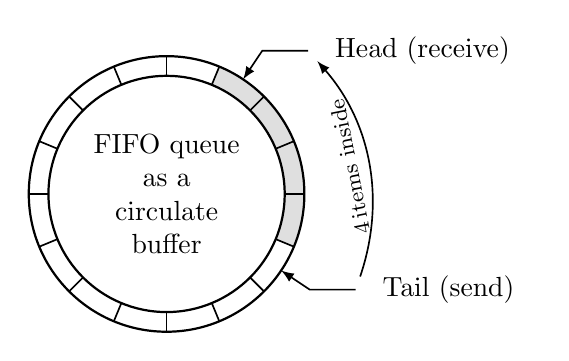
\begin{tikzpicture}[>=latex,semithick,scale=1.75]
        \fill [gray!25] (0,0) -- (67.5:1) arc [end angle=-22.5, start angle=67.5, radius=1] -- cycle;
        \draw [thick] (0,0) circle (1);
        \foreach \angle in {90,67.5,...,-67.5}
            \draw (\angle:1) -- (\angle-180:1);
        \node [circle,thick,fill=white,draw=black,align=center,minimum size=3cm] at (0,0) {FIFO queue\\ as a\\circulate \\buffer};
        \draw [<-] (56.25:1) -- (56.25:1.25) -- +(.333,0)
            node [right,inner xsep=.333cm] (Head) {Head (receive)};
        \draw [<-] (-33.75:1) -- (-33.75:1.25) -- +(.333,0)
            node [right,inner xsep=.333cm] (Tail) {Tail (send)};
        \draw [->,shorten >=5pt,shorten <=5pt] (Tail.west) to [bend right] 
            node [midway,sloped,above,allow upside down] {\footnotesize 4\,items inside}
        (Head.west);
    \end{tikzpicture}
    \caption{qQueues conceptual representation}
    \label{fig:qqueues}
\end{figure}

As showed in figure \ref{fig:qqueues}, the last position is connected back to the first position to make a circle. It is also called \textit{ring-buffer} or \textit{circular-queue}. 

In general, this kind of data structure is used to serialize data between tasks, allowing some elasticity in time. In many cases, the queue is used as a data buffer in interrupt service routines. This buffer will collect the data so, at some later time, another task can fetch the data for further processing. This use case is the single "task to task" buffering case. There are also other applications for queues as serializing  many data streams into one receiving streams (multiple tasks to a single task) or vice-versa (single task to multiple tasks).
The usage of this data structure is detailed in section \ref{queuecreate}.
\medskip
\begin{tcolorbox}
\ArrowBoldDownRight Note : The OS uses the queue by copy method. Queuing by copy is considered to be simultaneously more powerful and simpler to use than queuing by reference.
\end{tcolorbox}

Queuing by copy does not prevent the queue from also being used to queue by reference. For example, when the size of the data being queued makes it impractical to copy the data into the queue, then a pointer to the data can be copied into the queue instead.

\subsubsection{Event Flags}
Every task node has a set of built-in event bits called \textit{Event-Flags}, that can be used to indicate if an event has occurred or not.  
They are somewhat similar to signals, but with greater flexibility, providing a low cost, but flexible means of passing simple messages between tasks. One task can set or clear any combination of event flags. Another task may read the event flag group at any time or may wait for a specific pattern of flags.  
\begin{figure}[H]
    \centering
    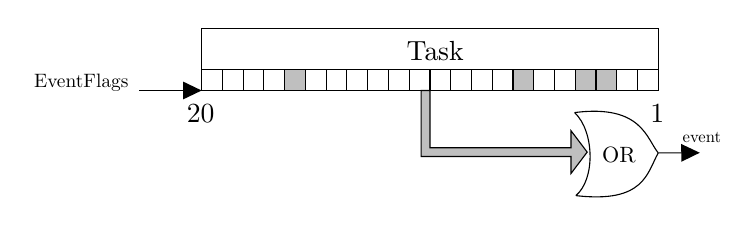
\begin{tikzpicture}[x=0.75pt,y=0.75pt,yscale=-1,xscale=1]
        \foreach \x in {100,110,...,270}{
            \draw   (\x,120) -- (\x+10,120) -- (\x+10,130) -- (\x,130) -- cycle ;
        }
        \draw  [fill=gray!50  ,fill opacity=1 ] (140,120) -- (150,120) -- (150,130) -- (140,130) -- cycle ;
        \draw  [fill=gray!50  ,fill opacity=1 ] (250,120) -- (260,120) -- (260,130) -- (250,130) -- cycle ;
        \draw  [fill=gray!50  ,fill opacity=1 ] (280,120) -- (290,120) -- (290,130) -- (280,130) -- cycle ;
        \draw  [fill=gray!50  ,fill opacity=1 ] (290,120) -- (300,120) -- (300,130) -- (290,130) -- cycle ;
        \draw   (300,120) -- (310,120) -- (310,130) -- (300,130) -- cycle ;
        \draw   (310,120) -- (320,120) -- (320,130) -- (310,130) -- cycle ;
        \draw   (100,100) -- (320,100) -- (320,120) -- (100,120) -- cycle ;
        \draw    (70,130) -- (79.5,130) -- (98,130) ;
        \draw [shift={(100,130)}, rotate = 180] [fill=black  ][line width=0.75]  [draw opacity=0] (8.93,-4.29) -- (0,0) -- (8.93,4.29) -- cycle    ;
        \draw    (320,160.06) .. controls (314.64,169.47) and (313.5,184.5) .. (280.29,180.64) ;
        \draw    (320,160.06) .. controls (314.4,153.47) and (312.16,136.5) .. (279.71,140.64) ;
        \draw    (280.29,180.64) .. controls (289.68,172.83) and (289.35,149.84) .. (279.71,140.64) ;
        \draw  [fill=gray!50  ,fill opacity=1 ] (210,130) -- (210,157.56) -- (277.94,157.56) -- (277.94,149.36) -- (285.75,159.68) -- (277.94,170) -- (277.94,161.8) -- (205.75,161.8) -- (205.75,130) -- cycle ;
        \draw    (320,160.06) -- (329.5,160.06) -- (338,160.01) ;
        \draw [shift={(340,160)}, rotate = 539.67] [fill=black ][line width=0.75]  [draw opacity=0] (8.93,-4.29) -- (0,0) -- (8.93,4.29) -- cycle    ;
        \draw (99.5,141) node  [align=left] {20};
        \draw (319.5,141) node  [align=left] {1};
        \draw (212.5,111) node  [align=left] {Task};
        \draw (42,126) node [scale=0.7] [align=left] {EventFlags};
        \draw (301,161) node [scale=0.8] [align=left] {OR};
        \draw (341,152.5) node [scale=0.6] [align=left] {event};
    \end{tikzpicture}
    \caption{Task event flags}
    \label{fig:eventflags}
\end{figure}

Up to twenty(20) bit-flags are available per task and whenever the scheduler sees that one event-flag is set, the kernel will trigger the task execution.

The function \lstinline{qTask_EventFlags_Modify} is intended to modify the task event-flags: 
\medskip

\begin{lstlisting}[style=CStyle]
void qTask_EventFlags_Modify( qTask_t * const Task, qTaskFlag_t flags, 
                              qBool_t action )
\end{lstlisting} \index{\lstinline{qTask_EventFlags_Modify}}

\subsubsection*{Parameters}
\begin{itemize}
    \item \lstinline{Task} : A pointer to the task node.
    \item \lstinline{flags} : The flags to modify. Can be combined with a bitwise \lstinline{OR} (\lstinline{|}).
    
    \lstinline{ QEVENTFLAG_01 | QEVENTFLAG_02 | QEVENTFLAG_03 | ... | QEVENTFLAG_20 }
    \item \lstinline{action} : \lstinline{QEVENTFLAG_SET} or \lstinline{QEVENTFLAG_CLEAR}. 
\end{itemize}

\begin{tcolorbox}
\HandRight The scheduler will put the task into a \textit{qReady} state when any of the available event-flags is set. The flags should be cleared by the application writer explicitly. 
\end{tcolorbox}

To read or check the event flags, the application can use one of the following API functions: 
\medskip

\begin{lstlisting}[style=CStyle]
qTaskFlag_t qTask_EventFlags_Read( const qTask_t * const Task )
\end{lstlisting} \index{\lstinline{qTask_EventFlags_Read}}

\subsubsection*{Parameters}
\begin{itemize}
    \item \lstinline{Task} : A pointer to the task node.
\end{itemize}

\subsubsection*{Return value:}

The EventFlag value of the task.

\noindent\hrulefill
\medskip

\begin{lstlisting}[style=CStyle]
qBool_t qTask_EventFlags_Check( qTask_t * const Task, 
                                qTaskFlag_t FlagsToCheck, 
                                qBool_t ClearOnExit, 
                                qBool_t CheckForAll )
\end{lstlisting} \index{\lstinline{qTask_EventFlags_Check}}

\subsubsection*{Parameters}
\begin{itemize}
    \item \lstinline{Task} : A pointer to the task node.
    \item \lstinline{FlagsToCheck} : A bitwise value that indicates the flags to test inside the EventFlags. Can be combined with a bitwise ‘OR’ (\lstinline{'|'}).
    \item \lstinline{ClearOnExit} : If is set to \lstinline{qTrue} then any flags set in the value passed as the \lstinline{FlagsToCheck} parameter will be cleared in the event group before this function returns only when the condition is meet.
    \item \lstinline{CheckForAll} : Used to create either a logical AND test (where all flags must be set)or a logical OR test (where one or more flags must be set) as follows:
    
    If is set to \lstinline{qTrue} this API will return \lstinline{qTrue} when all the flags set in the value passed as the \lstinline{FlagsToCheck} parameter are set in the task's EventFlags.
    
    If is set to \lstinline{qFalse} this API will return \lstinline{qTrue} when any of the flags set in the value passed as the \lstinline{FlagsToCheck} parameter are set in the task's EventFlags.

\end{itemize}

\subsubsection*{Return value:}

\lstinline{qTrue} if the condition is meet, otherwise return \lstinline{qFalse}.


\subsection{Retrieving the event data} \label{eventdata} \index{\lstinline{qEvent_t}}
As you can read in the previous sections, tasks can be triggered from multiple event sources (time-elapsed, notifications, queues and event-flags). This can lead to several situations that must be handled by the application writer from the task context, for example:

\begin{itemize}
    \item What is the event source that triggers the task execution?
    \item How to get the event associated data?
    \item What is the task execution status? 
\end{itemize}

The OS provides a simple approach for this, a data structure with all the regarding information of the task execution. This structure, that is already defined in the callback function as the \lstinline{qEvent_t} argument, is filled by the kernel dispatcher, so the application writer only needs to read the fields inside.

This data structure is defined as: 
\medskip

\begin{lstlisting}[style=CStyle]
typedef struct{
    qTrigger_t Trigger;
    void *TaskData;
    void *EventData;
    qBool_t FirstCall, FirstIteration, LastIteration;
    qClock_t StartDelay;
}qEvent_t;
\end{lstlisting}

Each field of the structure is described as follows
\begin{itemize}
    \item \lstinline{Trigger} : The flag that indicates the event source that triggers the task execution. This flag can only have nine(9) possible values:
    \begin{itemize}
        \item \lstinline{byTimeElapsed}  : When the time specified for the task elapsed.
        \item \lstinline{byNotificationQueued} : When there is a queued notification in the FIFO priority queue. For this trigger, the dispatcher performs a dequeue operation automatically. A pointer to the dequeued event-data will be available in the \lstinline{EventData}  field.
        \item \lstinline{byNotificationSimple} : When an asynchronous notification event  arrives by the usage of \lstinline{qTask_Notification_Send}. A pointer to the notification data will be available in the \lstinline{EventData} field.
        \item \lstinline{byQueueReceiver} : When there are elements available in the attached queue, the scheduler makes a data dequeue(auto-receive) from the front. A pointer to the received data will be available in the \lstinline{EventData} field.
        \item \lstinline{byQueueFull} : When the attached queue is full. A pointer to the queue will be available in the \lstinline{EventData} field.
        \item \lstinline{byQueueCount} : When the element-count of the  attached queue reaches
        the specified value. A pointer to the queue will be available in the \lstinline{EventData} field.
        \item \lstinline{byQueueEmpty} : When the attached queue is empty. A pointer to the queue will be available in the \lstinline{EventData} field.
        \item \lstinline{byEventFlags} : When any of the available event flags is set. Flags should be cleared by the application writer.
        \item \lstinline{byNoReadyTasks} : Only when the idle task is triggered
    \end{itemize}
    \item \lstinline{TaskData} : The storage pointer. Tasks can store a pointer to specific variable, structure or array, which represents specific user data for a particular task. This may be needed if you plan to use the same callback method for multiple tasks.
    \item \lstinline{EventData} : Associated data of the event. Specific data will reside here according to the event source. This field will have a \lstinline{NULL} value when the trigger gets one of this values:  \textit{byTimeElapsed}, \textit{byEventFlags} and \textit{byNoReadyTasks}.
    \item \lstinline{FirstCall} : This flag indicates that a task is running for the first time. Can be used for data initialization purposes.
    \item \lstinline{FirstIteration} : Indicates whether current pass is the first iteration of the task. This flag will be only set when time-elapsed events occurs and the iteration counter has been parameterized. 
    \item \lstinline{LastIteration} : Indicates whether current pass is the last iteration of the task. This flag will be only set when time-elapsed events occurs and the iteration counter has been parameterized. 
    \item \lstinline{StartDelay} : The number of epochs between current system time and point in time when the task was marked as Ready.
    Can be used to keep track when current task's execution took place relative to when it was scheduled. A value of 0 (zero) indicates that task started right on time per schedule.
    This parameter will be only available on timed tasks, when \lstinline{Trigger} \lstinline{==} \textit{byTimeElapsed}. 
\end{itemize}    

\begin{tcolorbox}
\HandRight Asynchronous events never change the task iteration counter, consequently, it has no effect on related fields, \lstinline{FirstIteration} and \lstinline{LastIteration}.
\end{tcolorbox}
    
\subsection{Implementation guidelines}
\subsubsection{Sending notifications}

The kernel handles all the notifications by itself (simple or queued), so intermediate objects aren't needed. Just calling \lstinline{qTask_Notification_Send()} or \lstinline{qTask_Notification_Queue()} is enough to send notifications. After the task callback is invoked, the notification is cleared by the dispatcher. Here the application writer must read the respective fields of the event-data structure to check the received notification. 
\medskip
The next example shows an ISR to task communication. Two interrupts send notifications to a single task with specific event data. The receiver task (\lstinline{taskA}) after further processing, send an event to \lstinline{taskB} to handle the event generated by the transmitter (\lstinline{taskA}).

\begin{lstlisting}[style=CStyle]
#include <stdio.h>
#include <stdlib.h>
#include <string.h>
#include "HAL.h" /*hardware dependent code*/
#include "QuarkTS.h"

qTask_t taskA, taskB;
void taskA_Callback( qEvent_t e );
void taskB_Callback( qEvent_t e );

const char *app_events[] = {
                            "Timer1seg", 
                            "ButtonRisingEdge", 
                            "ButtonFallingEdge", 
                            "3Count_ButtonPush"
                            };

/*==================================================================*/
void interrupt Timer1Second_ISR( void) {
    qTask_Notification_Send( &taskA, NULL );
    HAL_ClearInterruptFlags( HAL_TMR_ISR ); /*hardware dependent code*/
}
/*==================================================================*/
void interrupt ExternalInput_ISR( void ){
    if( RISING_EDGE == HAL_GetInputEdge() ){ /*hardware dependent code*/
        qTask_Notification_Queue( &taskA, app_events[1] );    
    }
    else{
        qTask_Notification_Queue( &taskA, app_events[2] );
    }
    HAL_ClearInterruptFlags( HAL_EXT_ISR ); /*hardware dependent code*/
}
/*==================================================================*/
void taskA_Callback( qEvent_t e ){
    static int press_counter = 0;
    
    switch(e->Trigger){ /*check the source of the event*/
        case byNotificationSimple: 
            /*
            * Do something here to process the timer event
            */
            break;
        case byNotificationQueued:
            /*here, we only care the Falling Edge events*/
            if( strcmp( e->EventData, "ButtonFallingEdge" )==0 ){
                press_counter++; /*count the button press*/
                if( press_counter == 3){ /*after 3 presses*/
                    /*send the notification of 3 presses to taskB*/
                    qTask_Notification_Send( &taskB, app_events[3] );
                    press_counter = 0;
                }
            }
            break;
        default:
            break;
    }
}
/*==================================================================*/
void taskB_Callback( qEvent_t e ){
    if( byNotificationSimple == e->Trigger){
        /*
         * we can do more here, but this is just an example,
         * so, this task will only print out the received 
         * notification event.
         */
        qDebug( e->EventData, Message );
    }
}
/*==================================================================*/
int main( void ){
    HAL_Setup_MCU(); /*hardware dependent code*/
    qTrace_Set_OutputFcn( HAL_OutPutChar );
    /* setup the scheduler to handle up to 10 queued notifications*/
    qOS_Setup( HAL_GetTick, 0.001, NULL ); 
    qOS_Add_EventTask( &taskA, taskA_Callback, qLowest_Priority, NULL );
    qOS_Add_EventTask( &taskB, taskB_Callback, qLowest_Priority, NULL );                     
    qOS_Run();
    return 0;
}
\end{lstlisting}

\subsubsection{Setting up a queue : \texorpdfstring{\lstinline{qQueue_Setup}}{qQueue_Setup} } \index{\lstinline{qQueue_Setup}} \label{queuecreate}
A queue must be explicitly initialized before it can be used. 
\medskip
These objects are referenced by handles, which are variables of type \lstinline{qQueue_t}. The \lstinline{qQueue_Setup()} API function configures the queue and initialize the instance. 

The required RAM for the queue data should be provided by the application writer and could be statically allocated at compile time or in run-time using the memory management module.
\medskip
 
\begin{lstlisting}[style=CStyle]
qBool_t qQueue_Setup( qQueue_t * const obj, void* DataArea, 
                      size_t ItemSize, size_t ItemsCount )
\end{lstlisting}

\subsubsection*{Parameters}
\begin{itemize}
    \item \lstinline{obj} : A pointer to the queue object
    \item \lstinline{DataArea} : Must point to a data block or array of data that is at least large enough to hold the maximum number of items that can be in the queue at any one time
    \item \lstinline{ItemSize} : Size of one element in the data block
    \item \lstinline{ItemsCount} : The maximum number of items the queue can hold at any one time.
\end{itemize}      
    
\noindent\hrulefill    
    
\subsubsection{Performing queue operations}
\index{\lstinline{qQueue_SendToBack}}
\begin{lstlisting}[style=CStyle]
qBool_t qQueue_SendToBack( qQueue_t * const obj, void *ItemToQueue )
\end{lstlisting}

\index{\lstinline{qQueue_SendToFront}}
\begin{lstlisting}[style=CStyle]
qBool_t qQueue_SendToFront( qQueue_t * const obj, void *ItemToQueue )
\end{lstlisting}

As might be expected, \lstinline{qQueue_SendToBack()} is used to send data to the back (tail) of a queue, and \lstinline{qQueue_SendToFront()} is used to send data to the front (head) of a queue. \lstinline{qQueue_Send()} \index{\lstinline{qQueue_Send}} is equivalent to, and exactly the same as, \lstinline{qQueue_SendToBack()}.

\subsubsection*{Parameters}
\begin{itemize}
    \item \lstinline{obj} : A pointer to the queue object
    \item \lstinline{ItemToQueue} : A pointer to the item that is to be placed on the queue. The size of the items the queue will hold was defined when the queue was created, so this many bytes will be copied from \lstinline{ItemToQueue} into the queue storage area. 
\end{itemize}  

\subsubsection*{Return value}
\lstinline{qTrue} if data was retrieved from the queue, otherwise returns \lstinline{qFalse}.

\noindent\hrulefill  

The API \lstinline{qQueue_Receive()} \index{\lstinline{qQueue_Receive}} is used to receive (read) an item from a queue. The item that is received is removed from the queue. 
\medskip

\begin{lstlisting}[style=CStyle]
qBool_t qQueue_Receive( qQueue_t * const obj, void *dest )
\end{lstlisting}

\subsubsection*{Parameters}
\begin{itemize}
    \item \lstinline{obj} : A pointer to the queue object
    \item \lstinline{ItemToQueue} : Pointer to the buffer into which the received item will be copied.
\end{itemize}  

\subsubsection*{Return value}
\lstinline{qTrue} if data was retrieved from the queue, otherwise returns \lstinline{qFalse}.

\subsubsection{Attach a queue to a task}
Additional features are provided by the kernel when the queues are attached to tasks; this allows the scheduler to pass specific queue events to it, usually, states of the object itself that needs to be handled, in this case by a task. For this, the following API is provided: \index{\lstinline{qTask_Attach_Queue}} 
\medskip
    
\begin{lstlisting}[style=CStyle]
qBool_t qTask_Attach_Queue( qTask_t * const Task, qQueue_t * const Queue,
                            const qQueue_LinkMode_t Mode, 
                            const qUINT16_t arg )
\end{lstlisting}
    
\subsubsection*{Parameters}
\begin{itemize}
    \item \lstinline{Task} : A pointer to the task node
    \item \lstinline{Queue} : A pointer to the queue object
    \item \lstinline{Mode} : Attach mode. This implies the event that will trigger the task according to one of the following modes:
    \begin{itemize}
        \item \lstinline{qQUEUE_DEQUEUE} : The task will be triggered if there are elements in the queue. 
        \item \lstinline{qQUEUE_FULL} :  The task will be triggered if the queue is full. 
        \item \lstinline{qQUEUE_COUNT} :  The task will be triggered if the count of elements in the queue reach the specified value. 
        \item \lstinline{qQUEUE_EMPTY} :  The task will be triggered if the queue is empty.
    \end{itemize}
    \item \lstinline{arg} : This argument defines if the queue will be attached (\lstinline{qATTACH}) or detached (\lstinline{qDETACH}) from the task. If the \lstinline{qQUEUE_COUNT} mode is specified, this value will be used to check the element count of the queue. A zero value will act as \lstinline{qDETACH} action. 
\end{itemize}  

\begin{tcolorbox}
\HandRight For the \lstinline{qQUEUE_DEQUEUE} mode,  data from the front of the queue will be received automatically in every trigger, this involves a data removal after the task is served. During the respective task execution, the \lstinline{EventData} field of the \lstinline{qEvent_t} structure will be pointing to the extracted data. For the other modes, the \lstinline{EventData} field will point to the queue that triggered the event.
\end{tcolorbox}
    
\subsubsection{A queue example}
This example shows the usage of QuarkTS queues. The application is the classic producer/consumer example. The producer task puts data into the queue. When the queue reaches a specific item count, the consumer task is triggered to start fetching data from the queue. Here, both tasks are attached to the queue. 
\medskip

\begin{lstlisting}[style=CStyle]
#include <stdio.h>
#include <stdlib.h>
#include <stdint.h>
#include "QuarkTS.h"
#define TIMER_TICK   0.001   /* 1ms */ 

/*-----------------------------------------------------------------------*/
void interrupt Timer0_ISR( void ) {
    qClock_SysTick();   
}
/*-----------------------------------------------------------------------*/
qTask_t TSK_PRODUCER, TSK_CONSUMER; /*task nodes*/
qQueue_t UserQueue; /*Queue Handle*/
/*-----------------------------------------------------------------------*/

/* The producer task puts data into the buffer if there is enough free 
 * space in it, otherwise the task block itself and wait until the queue 
 * is empty to resume. */
void TSK_Producer_Callback( qEvent_t e ) {
    static qUINT16_t unData = 0;
    unData++;	
    /*Queue is empty, enable the producer if it was disabled*/
    if( byQueueEmpty == e->Trigger){
        qTask_Resume( qTask_Self() );
    }

    /*send data to the queue*/
    if( !qQueue_SendToBack( &UserQueue, &unData ) ){ 
        /*
        * if the data insertion fails, the queue is full 
        * and the task disables itself
        */
	    qTask_Suspend( qTask_Self() ); 
    }
}
/*-----------------------------------------------------------------------*/
/* The consumer task gets one element from the queue.*/
void TSK_Consumer_Callback( qEvent_t e ) {
    qUINT16_t unData;
    qQueue_t *ptrQueue; /*a pointer to the queue that triggers the event*/
    if( byQueueCount == e->Trigger ){
	    ptrQueue= (qQueue_t *)e->EventData;
	    qQueue_Receive( ptrQueue, &unData );
	    return;
    }
}
/*-----------------------------------------------------------------------*/
void IdleTask_Callback( qEvent_t e ){
    /*nothing to do...*/
}	
/*-----------------------------------------------------------------------*/
int main( void ) {    
    qUINT8_t BufferMem[ 16*sizeof(qUINT16_t) ] = {0};  
    HardwareSetup();  //hardware specific code
    /* next line is used to setup hardware with specific code to fire
     * interrupts at 1ms - timer tick*/
    Configure_Periodic_Timer0_Interrupt_1ms();
 
    qOS_Setup( NULL, TIMER_TICK, IdleTask_Callback );     
    /*Setup the queue*/
    qQueue_Setup( &UserQueue, BufferMem /*Memory block used*/, 
                  sizeof(qUINT16_t) /*element size*/, 
                  16 /* element count*/ );     
                 
    /*  Append the producer task with 100mS rate. */
    qOS_Add_Task( &TSK_PRODUCER, TSK_Producer_Callback, 
                  qMedium_Priority, 0.1, qPeriodic, qEnabled, 
                  "producer" );
    /* Append the consumer as an event task. The consumer will
     * wait until an event trigger their execution
     */
    qOS_Add_EventTask( &TSK_CONSUMER, TSK_Consumer_Callback,
                       qMedium_Priority, "consumer" );
    /* the queue will be attached to the consumer task 
     * in qQUEUE_COUNT mode. This mode sends an event to the consumer
     * task when the queue fills to a level of 4 elements
     */
    qTask_Attach_Queue( &TSK_CONSUMER, &UserQueue, qQUEUE_COUNT, 4 );
    /* the queue will be attached to the producer task in
     * qQUEUE_EMPTY mode. This mode sends an event to the producer
     * task when the queue is empty
     */
     
    qTask_Attach_Queue( &TSK_PRODUCER, &UserQueue, qQUEUE_EMPTY, qATTACH );
    qOS_Run();
    return 0;
}

\end{lstlisting}    

\subsubsection{Other queue APIs}

\begin{lstlisting}[style=CStyle]
void qQueue_Reset( qQueue_t * const obj )
\end{lstlisting}

Resets a queue to its original empty state. \index{\lstinline{qQueue_Reset}}

\subsubsection*{Parameters:}
\begin{itemize}
    \item \lstinline{obj} : A pointer to the queue object
\end{itemize}

\noindent\hrulefill


\begin{lstlisting}[style=CStyle]
qBool_t qQueue_IsEmpty( const qQueue_t * const obj );
\end{lstlisting}

Returns the empty status of the queue. \index{\lstinline{qQueue_IsEmpty}}

\subsubsection*{Parameters:}
\begin{itemize}
    \item \lstinline{obj} : A pointer to the queue object
\end{itemize}

\subsubsection*{Return value:}
\lstinline{qTrue} if the queue is empty, \lstinline{qFalse} if it is not.

\noindent\hrulefill


\begin{lstlisting}[style=CStyle]
size_t qQueue_Count( const qQueue_t * const obj )
\end{lstlisting}

Returns the number of items in the queue. \index{\lstinline{qQueue_Count}}

\subsubsection*{Parameters:}
\begin{itemize}
    \item \lstinline{obj} : A pointer to the queue object.
\end{itemize}

\subsubsection*{Return value:}
The number of elements in the queue.

\noindent\hrulefill


\begin{lstlisting}[style=CStyle]
qBool_t qQueue_IsFull( const qQueue_t * const obj )
\end{lstlisting}

Returns the full status of the queue. \index{\lstinline{qQueue_IsFull}}

\subsubsection*{Parameters:}
\begin{itemize}
    \item \lstinline{obj} : A pointer to the queue object.
\end{itemize}

\subsubsection*{Return value:}
\lstinline{qTrue} if the queue is full, \lstinline{qFalse} if it is not.

\noindent\hrulefill


\begin{lstlisting}[style=CStyle]
void* qQueue_Peek( const qQueue_t * const obj )
\end{lstlisting}

Looks at the data from the front of the queue without removing it. \index{\lstinline{qQueue_Peek}}  

\subsubsection*{Parameters:}
\begin{itemize}
    \item \lstinline{obj} : A pointer to the queue object.
\end{itemize}

\subsubsection*{Return value:}
Pointer to the data, or \lstinline{NULL} if there is nothing in the queue.

\noindent\hrulefill


\begin{lstlisting}[style=CStyle]
qBool_t qQueue_RemoveFront( qQueue_t * const obj )
\end{lstlisting}

Remove the data located at the front of the queue. \index{\lstinline{qQueue_RemoveFront}}

\subsubsection*{Parameters:}
\begin{itemize}
    \item \lstinline{obj} : A pointer to the queue object.
\end{itemize}

\subsubsection*{Return value:}
\lstinline{qTrue} if data was removed from the queue, otherwise returns \lstinline{qFalse}.

\subsubsection{Using the task Event-flags}
This example demonstrate the usage of \textit{Event-flags}. The idle task will transmit data generated from another task, only when the required conditions are met, including two events from an ISR (A timer expiration and the change of a digital input) and when a new set of data is generated.
The task that generates the data should wait until the idle task transmission is done to generate a new data set. 
\medskip

\begin{lstlisting}[style=CStyle]
#include <stdio.h>
#include <stdlib.h>
#include <stdint.h>
#include "QuarkTS.h"
#define TIMER_TICK   0.001   /* 1ms */ 

/*event flags application definitions */
#define SWITCH_CHANGED  QEVENTFLAG_01
#define TIMER_EXPIRED   QEVENTFLAG_02
#define DATA_READY      QEVENTFLAG_03
#define DATA_TXMIT      QEVENTFLAG_04

qTask_t TaskDataProducer; 
qUINT8_t dataToTransmit[10] = {0};

/*-----------------------------------------------------------------------*/
void interrupt Timer0_ISR( void ){
    qClock_SysTick();   
}
/*-----------------------------------------------------------------------*/
void interrupt Timer1_ISR( void ){
    qTask_EventFlags_Modify( &TaskDataProducer, TIMER_EXPIRED, 
                             QEVENTFLAG_SET );
}
/*-----------------------------------------------------------------------*/
void interrupt EXTI_ISR( void ){
    if( EXTI_IsRisingEdge() ){
        qTask_EventFlags_Modify( &TaskDataProducer, SWITCH_CHANGED, 
                                 QEVENTFLAG_SET );
    }
}
/*-----------------------------------------------------------------------*/
void TaskDataProducer_Callback( qEvent_t e ){
    qBool_t condition;
    condition = qTask_EventFlags_Check( &TaskDataProducer, 
                                        DATA_TXMIT, qTrue, qTrue );
    if( qTrue == condition){
        GenerateData( dataToTransmit );
        qTask_EventFlags_Modify( &TaskDataProducer, DATA_READY, 
                                 QEVENTFLAG_SET ); 
    }
    qTask_EventFlags_Check( &TaskDataProducer, 
                            DATA_READY | SWITCH_CHANGED | TIMER_EXPIRED,
                            qTrue, qTrue );
}
/*-----------------------------------------------------------------------*/
void IdleTask_Callback( qEvent_t e ){
    
    TransmitData( dataToTransmit );
    qTask_EventFlags_Modify( &TaskDataProducer, 
                             DATA_TXMIT, QEVENTFLAG_SET ); 
}
/*-----------------------------------------------------------------------*/
int main( void ) {    
    HardwareSetup();  //hardware specific code
    /* next line is used to setup hardware with specific code to fire
     * interrupts at 1ms - timer tick*/
    Configure_Periodic_Timer0_Interrupt_1ms();
    Configure_Periodic_Timer1_Interrupt_2s();
    Configure_External_Interrupt();
    /*
    Idle task will be responsible to transmit the generate the data after 
    all conditions are meet
    */
    qOS_Setup( NULL, TIMER_TICK, IdleTask_Callback );
    /*
    The task will wait until data is transmitted to generate another set of
    data
    */
    qOS_Add_EventTask( &TaskDataProducer, TaskDataProducer_Callback,
                       qHigh_Priority, "DATAPRODUCER" );
    /*
    Set the flag DATA_TXMIT as initial condition to allow the data 
    generation at startup
    */
    qTask_EventFlags_Modify( &TaskDataProducer, DATA_TXMIT, QEVENTFLAG_SET ); 
    qOS_Run();
    for(;;){}
    return 0;
}

\end{lstlisting}

\newpage
